\begin{frame}
\setbeamercovered{invisible}
\begin{adjustwidth}{-2.3em}{-2.5em}

% Set the overall layout of the tree
\tikzstyle{level 1}=[level distance=8em, sibling distance=10.8em]
\tikzstyle{level 2}=[level distance=11em, sibling distance=4.3em]

% Define styles
\tikzstyle{root} = [minimum width=12mm, minimum height=8mm]
\tikzstyle{internal} = [minimum width=12mm, minimum height=8mm]
\tikzstyle{tip} = [minimum width=12mm, minimum height=8mm]
\tikzstyle{branch} = [->, very thick]

\vspace{-2mm}
\uncover<6->{
\hspace{0.5\textwidth}
    {\LARGE $\boldsymbol{\alpha =} \only<6>{\mathbf{\conc}}\only<7->{\mathbf{\cconc}}$} \\
}

\vspace{5mm}

\noindent
\begin{tikzpicture}[grow=right]%, sloped]
\pgfkeys{/pgf/number format/.cd,fixed,fixed zerofill,precision=3}
\node[root] {\pgftext{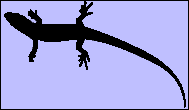
\includegraphics[width=8mm]{../images/dpp-node-1.pdf}}}
    child [visible on=<2->]{
        node[internal] {\pgftext{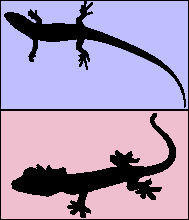
\includegraphics[width=8mm]{../images/dpp-node-12.pdf}}}        
            child [visible on=<4->]{
                node[tip, label=right:
                    {\tiplabel{\uncover<5->{
                        $
                        % p(m = 123)=
                        \left(\frac{\alpha}{\alpha+1}\right)\left(\frac{\alpha}{\alpha+2}\right)
                        \only<6>{= \calcprob{\conc}{\conc}}
                        \uncover<7->{= \ccalcprob{\cconc}{\cconc}}$
                        }}}]
                    {\pgftext{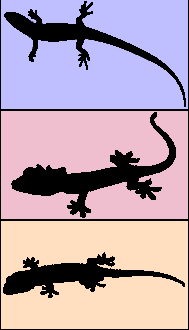
\includegraphics[width=8mm]{../images/dpp-node-123.pdf}}}
                edge from parent [style = branch]
                node[above,
                    label={[label distance = -0.7em]\branchlabel{$\frac{\alpha}{\alpha+2}$}}
                    ] {}
            }
            child [visible on=<4->]{
                node[tip, label=right:
                    {\tiplabel{\uncover<5->{
                        $
                        % p(m = 121)=
                        \left(\frac{\alpha}{\alpha+1}\right)\left(\frac{1}{\alpha+2}\right)
                        \only<6>{= \calcprob{\conc}{1}}
                        \uncover<7->{= \ccalcprob{\cconc}{1}}$
                        }}}]
                    {\pgftext{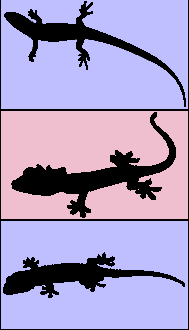
\includegraphics[width=8mm]{../images/dpp-node-121.pdf}}}
                edge from parent [style = branch]
                node[above,
                    label={[label distance = -0.7em]\branchlabel{$\frac{1}{\alpha+2}$}}
                    ] {}
            }
            child [visible on=<4->]{
                node[tip, label=right:
                    {\tiplabel{\uncover<5->{
                        $
                        % p(m = 122)=
                        \left(\frac{\alpha}{\alpha+1}\right)\left(\frac{1}{\alpha+2}\right)
                        \only<6>{= \calcprob{\conc}{1}}
                        \uncover<7->{= \ccalcprob{\cconc}{1}}$
                        }}}]
                    {\pgftext{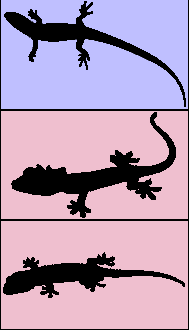
\includegraphics[width=8mm]{../images/dpp-node-122.pdf}}}
                edge from parent [style = branch]
                node[above,
                    label={[label distance = -0.5em]\branchlabel{$\frac{1}{\alpha+2}$}}
                    ] {}
            }
            edge from parent [style = branch]
            node[above,
                label={[label distance = 0em]\branchlabel{$\frac{\alpha}{\alpha+1}$}}
                ] {}
    }
    child [visible on=<2->]{
        node[internal] {\pgftext{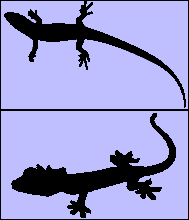
\includegraphics[width=8mm]{../images/dpp-node-11.pdf}}}        
            child [visible on=<3->]{
                node[tip, label=right:
                    {\tiplabel{\uncover<5->{
                        $
                        % p(m = 112)=
                        \left(\frac{1}{\alpha+1}\right)\left(\frac{\alpha}{\alpha+2}\right)
                        \only<6>{= \calcprob{1}{\conc}}
                        \uncover<7->{= \ccalcprob{1}{\cconc}}$
                        }}}]
                    {\pgftext{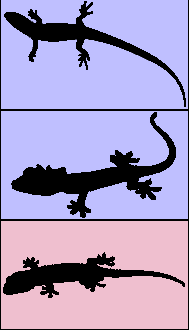
\includegraphics[width=8mm]{../images/dpp-node-112.pdf}}}
                edge from parent [style = branch]
                node[above,
                    label={[label distance = -0.7em]\branchlabel{$\frac{\alpha}{\alpha+2}$}}
                    ] {}
            }
            child [visible on=<3->]{
                node[tip, label=right:
                    {\tiplabel{\uncover<5->{
                        $
                        % p(m = 111)=
                        \left(\frac{1}{\alpha+1}\right)\left(\frac{2}{\alpha+2}\right)
                        \only<6>{= \calcprob{1}{2}}
                        \uncover<7->{= \ccalcprob{1}{2}}$
                        }}}]
                    {\pgftext{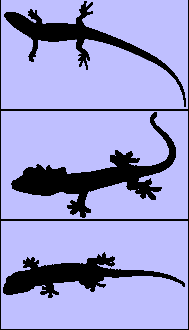
\includegraphics[width=8mm]{../images/dpp-node-111.pdf}}}
                edge from parent [style = branch]
                node[above,
                    label={[label distance = -0.7em]\branchlabel{$\frac{2}{\alpha+2}$}}
                    ] {}
            }
            edge from parent [style = branch]
            node[above,
                label={[label distance = 0em]\branchlabel{$\frac{1}{\alpha+1}$}}
                ] {}
    };
\end{tikzpicture}

\end{adjustwidth}
\end{frame}

